\definecolor{aa}{RGB}{227,26,28}
\definecolor{ab}{RGB}{56,125,184}
\definecolor{ac}{RGB}{77,176,74}
\definecolor{ak}{RGB}{0,0,0}

% GNUPLOT: LaTeX picture with Postscript
\begingroup
  \makeatletter
  \providecommand\color[2][]{%
    \GenericError{(gnuplot) \space\space\space\@spaces}{%
      Package color not loaded in conjunction with
      terminal option `colourtext'%
    }{See the gnuplot documentation for explanation.%
    }{Either use 'blacktext' in gnuplot or load the package
      color.sty in LaTeX.}%
    \renewcommand\color[2][]{}%
  }%
  \providecommand\includegraphics[2][]{%
    \GenericError{(gnuplot) \space\space\space\@spaces}{%
      Package graphicx or graphics not loaded%
    }{See the gnuplot documentation for explanation.%
    }{The gnuplot epslatex terminal needs graphicx.sty or graphics.sty.}%
    \renewcommand\includegraphics[2][]{}%
  }%
  \providecommand\rotatebox[2]{#2}%
  \@ifundefined{ifGPcolor}{%
    \newif\ifGPcolor
    \GPcolorfalse
  }{}%
  \@ifundefined{ifGPblacktext}{%
    \newif\ifGPblacktext
    \GPblacktexttrue
  }{}%
  % define a \g@addto@macro without @ in the name:
  \let\gplgaddtomacro\g@addto@macro
  % define empty templates for all commands taking text:
  \gdef\gplbacktext{}%
  \gdef\gplfronttext{}%
  \makeatother
  \ifGPblacktext
    % no textcolor at all
    \def\colorrgb#1{}%
    \def\colorgray#1{}%
  \else
    % gray or color?
    \ifGPcolor
      \def\colorrgb#1{\color[rgb]{#1}}%
      \def\colorgray#1{\color[gray]{#1}}%
      \expandafter\def\csname LTw\endcsname{\color{white}}%
      \expandafter\def\csname LTb\endcsname{\color{black}}%
      \expandafter\def\csname LTa\endcsname{\color{black}}%
      \expandafter\def\csname LT0\endcsname{\color[rgb]{1,0,0}}%
      \expandafter\def\csname LT1\endcsname{\color[rgb]{0,1,0}}%
      \expandafter\def\csname LT2\endcsname{\color[rgb]{0,0,1}}%
      \expandafter\def\csname LT3\endcsname{\color[rgb]{1,0,1}}%
      \expandafter\def\csname LT4\endcsname{\color[rgb]{0,1,1}}%
      \expandafter\def\csname LT5\endcsname{\color[rgb]{1,1,0}}%
      \expandafter\def\csname LT6\endcsname{\color[rgb]{0,0,0}}%
      \expandafter\def\csname LT7\endcsname{\color[rgb]{1,0.3,0}}%
      \expandafter\def\csname LT8\endcsname{\color[rgb]{0.5,0.5,0.5}}%
    \else
      % gray
      \def\colorrgb#1{\color{black}}%
      \def\colorgray#1{\color[gray]{#1}}%
      \expandafter\def\csname LTw\endcsname{\color{white}}%
      \expandafter\def\csname LTb\endcsname{\color{black}}%
      \expandafter\def\csname LTa\endcsname{\color{black}}%
      \expandafter\def\csname LT0\endcsname{\color{black}}%
      \expandafter\def\csname LT1\endcsname{\color{black}}%
      \expandafter\def\csname LT2\endcsname{\color{black}}%
      \expandafter\def\csname LT3\endcsname{\color{black}}%
      \expandafter\def\csname LT4\endcsname{\color{black}}%
      \expandafter\def\csname LT5\endcsname{\color{black}}%
      \expandafter\def\csname LT6\endcsname{\color{black}}%
      \expandafter\def\csname LT7\endcsname{\color{black}}%
      \expandafter\def\csname LT8\endcsname{\color{black}}%
    \fi
  \fi
    \setlength{\unitlength}{0.0500bp}%
    \ifx\gptboxheight\undefined%
      \newlength{\gptboxheight}%
      \newlength{\gptboxwidth}%
      \newsavebox{\gptboxtext}%
    \fi%
    \setlength{\fboxrule}{0.5pt}%
    \setlength{\fboxsep}{1pt}%
\begin{picture}(5000.00,5000.00)%
    \gplgaddtomacro\gplbacktext{%
      \colorrgb{0.15,0.15,0.15}%
      \put(391,1564){\makebox(0,0)[r]{\strut{}$6.0$}}%
      \colorrgb{0.15,0.15,0.15}%
      \put(391,1988){\makebox(0,0)[r]{\strut{}$8.0$}}%
      \colorrgb{0.15,0.15,0.15}%
      \put(391,2413){\makebox(0,0)[r]{\strut{}$10.0$}}%
      \colorrgb{0.15,0.15,0.15}%
      \put(391,2837){\makebox(0,0)[r]{\strut{}$12.0$}}%
      \colorrgb{0.15,0.15,0.15}%
      \put(391,3262){\makebox(0,0)[r]{\strut{}$14.0$}}%
      \colorrgb{0.15,0.15,0.15}%
      \put(391,3687){\makebox(0,0)[r]{\strut{}$16.0$}}%
      \colorrgb{0.00,0.00,0.00}%
      \put(672,1280){\makebox(0,0){\strut{}$-2.0$}}%
      \colorrgb{0.00,0.00,0.00}%
      \put(1096,1280){\makebox(0,0){\strut{}$0.0$}}%
      \colorrgb{0.00,0.00,0.00}%
      \put(1521,1280){\makebox(0,0){\strut{}$2.0$}}%
      \colorrgb{0.00,0.00,0.00}%
      \put(1945,1280){\makebox(0,0){\strut{}$4.0$}}%
      \colorrgb{0.00,0.00,0.00}%
      \put(2370,1280){\makebox(0,0){\strut{}$6.0$}}%

      \put(1120,4104){\makebox(0,0){\strut{}{\color{ak}{\rule[0.6mm]{0.5cm}{0.5mm}}} \footnotesize sensor trajectory}}
      \put(2470,4104){\makebox(0,0){\strut{}{\color{aa}{\rule[0.6mm]{0.5cm}{0.5mm}}} \footnotesize CSM}}
      \put(3370,4104){\makebox(0,0){\strut{}{\color{ab}{\rule[0.6mm]{0.5cm}{0.5mm}}} \footnotesize NDT}}
      \put(4240,4104){\makebox(0,0){\strut{}{\color{ac}{\rule[0.6mm]{0.5cm}{0.5mm}}} \footnotesize FSM}}
      \put(1500,1004){\makebox(0,0){\strut{} \footnotesize Frequent measurements}}
      \put(3600,1004){\makebox(0,0){\strut{} \footnotesize Infrequent measurements}}
    }%
    \gplgaddtomacro\gplfronttext{%
    }%
    \gplgaddtomacro\gplbacktext{%
      \colorrgb{0.00,0.00,0.00}%
      \put(2822,1280){\makebox(0,0){\strut{}$-2.0$}}%
      \colorrgb{0.00,0.00,0.00}%
      \put(3246,1280){\makebox(0,0){\strut{}$0.0$}}%
      \colorrgb{0.00,0.00,0.00}%
      \put(3671,1280){\makebox(0,0){\strut{}$2.0$}}%
      \colorrgb{0.00,0.00,0.00}%
      \put(4095,1280){\makebox(0,0){\strut{}$4.0$}}%
      \colorrgb{0.00,0.00,0.00}%
      \put(4520,1280){\makebox(0,0){\strut{}$6.0$}}%
    }%
    \gplgaddtomacro\gplfronttext{%
    }%
    \gplbacktext
    \put(0,0){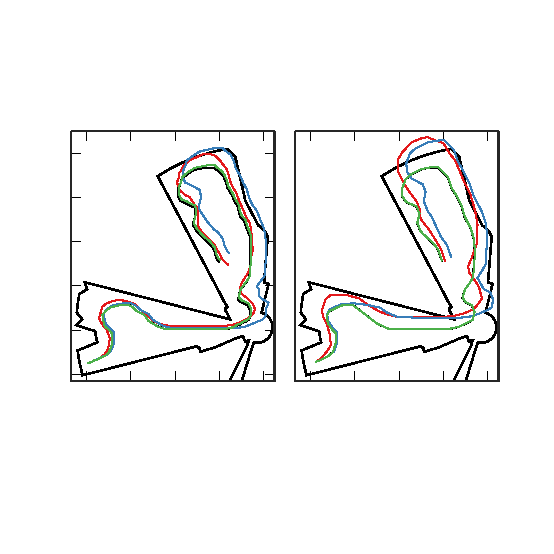
\includegraphics{./figures/odom_test_5_vs_6}}%
    \gplfronttext
  \end{picture}%
\endgroup
